\documentclass[annotation,times,page4]{itmo-student-thesis}

%% Опции пакета:
%% - annotation - если есть, генерируется аннотация, иначе не генерируется
%% - times - делает все шрифтом Times New Roman, требует пакета pscyr.
%% - page4 - начинает нумерацию оглавления с четвертой, а не с третьей страницы

%% Данные пакеты необязательны к использованию в бакалаврских/магистерских
%% Они нужны для иллюстративных целей
%% Начало
\usepackage{tikz}
\usetikzlibrary{arrows}
\usepackage{filecontents}
\begin{filecontents}{master-thesis.bib}
@inproceedings{ example-english,
    year        = {2016},
    booktitle   = {Proceedings of IEEE Congress on Evolutionary Computation},
    author      = {Maxim Buzdalov and Anatoly Shalyto},
    title       = {Hard Test Generation for Augmenting Path Maximum Flow 
                   Algorithms using Genetic Algorithms: Revisited},
    pages       = {2121-2128},
    langid      = {english}
}

@article{ example-russian,
    author      = {Максим Викторович Буздалов},
    title       = {Генерация тестов для олимпиадных задач по программированию 
                   с использованием генетических алгоритмов},
    journal     = {Научно-технический вестник {СПбГУ} {ИТМО}},
    number      = {2(72)},
    year        = {2011},
    pages       = {72-77},
    langid      = {russian}
}
@inproceedings{golbeck2011predicting,
  title={Predicting personality with social media},
  author={Golbeck, Jennifer and Robles, Cristina and Turner, Karen},
  booktitle={CHI'11 Extended Abstracts on Human Factors in Computing Systems},
  pages={253--262},
  year={2011},
  organization={ACM}
}
\end{filecontents}
%% Конец

%% Указываем файл с библиографией.
\addbibresource{master-thesis.bib}

\begin{document}

\studygroup{М4238}
\title{Выделение групп пользователей в социльных медиа по их интересам и поведению на основе множества истоников данных}
\author{Дмитриев С.С.}
\supervisor{Фильченков А.А.}
\supervisordegree{кандидат. техн. наук, доцент}
\publishyear{2016}

%% Транслируется в "Направление и задача исследований"
\researchdirections{Целью данного исследования является создание алгоритма выделения групп пользователей социальных сетей на основе их социальных связей и поведения в социальных сетях}

%% Транслируется в "Проектная и исследовательская часть"
\researchpart{В рамках данной работы предложен подход, позволяющий выделять подгруппы у выбранной группы пользователей в социальных сетях, основывающийся на социальных связах и видимом поведении на публичных страницах. В основе предложенного подхода лежат несколько методов и концепций: представление социальных связей в виде графа, случайные марковские поля, а так же семантический анализ. В качестве примера использования подхода взята группа футбольных болельщиков, и подгруппа радикальных футбольных болельщиков, а так же группа феменисток и подгруппа радикальных феменисток. Были использованы данные пользователей из социальной сети Vk.com. Достигнуты следущие показатели для группы футбольных болельщиков: ; для группы феменисток: . Данный подход нов и так же может применятся для других групп и подгрупп пользователей.}

%% Транслируется в "Экономическая часть"
\economicpart{Данная работа не прополагает извлечения экономической выгоды из полученных результатов}

%% Транслируется в "Характеристика вопросов экологии, техники безопасности"
\ecologypart{Результатом работы является программный продукт, не нарушающий 
требования экологической безопасности.}

%% Транслируется в "Новизна полученных результатов"
\novelty{В рамках описываемого исследования представлен подход позволяющий опредлять принадлежность пользователя к определенной группе на основе его социальных связей и публичного поведения в социальной сети. Полученный подход является способом построения модели, не применявшимся для решения подобной задачи ранее. }

%% Транслируется в "Является ли работа продолжением курсовых проектов, есть ли публикации"
\cwpublications{Работа не является продолжением курсовых проектов. На тему диссертации имеются публикации. //СПИСОК-2016//... потом дописать}

%% Транслируется в "Практическая ценность работы. Рекомендации по внедрению"
\practicalimplications{Полученный алгоритм дает возможность определить является ли член выбранной группы так же членом её подможества. Это может быть использовано правоохранительными органами, т.к. алгоритм позволяет выделить, например подгруппы, склонные к бандитизму, пользователей потенциально более способных на совершение незаконных действий, нежели среднестатистический пользователь. Так же алгоритм может быть использован для усовершенствования таргетированной рекламы, например для выделения подгруппы фанатов определенного брэнда из группы его покупаетелей.}

%% Эта команда генерирует титульный лист и аннотацию.
\makemastertitle

%% Оглавление
\tableofcontents

%% Макрос для введения. Совместим со старым стилевиком.
\startprefacepage

Последнее время социальные медиа набрали огромную популярность. Такие сайты как Facebook.com, Vk.com, Twitter.com, обладают огромной аудиторией. Совокупный размер аудитории существующих социальных сетей составляет более двух миллиардов пользователей и их число постоянно растет. Они создают огромные массы контента, состоящего из их мнений и точек зрения. Так в течении суток на Facebook.com более 4.5 миллиардов раз пользователи ставят лайки, оставляют более 700 тысяч публичных комментариев, публикуют более 100 миллионов фотографий. Однако содержание этой информации в основном остается не исползованным. Тогда как оно может быть крайне важным.

Такие данные могут быть использованы для определения интересов, предпочтений и иных личных свойств пользователя. Часть подобной информации, пол, возраст,  местоположение, увлечения, может быть указана в профиле пользователя. Однако, зачастую, таки данные могут быть неполными, а иногда и неверными. А некоторые признаки, например, вероисповедание, политические взгляды или же принадлежность к неким общественным движениям обычно опускаются. Из-за этой неполноты возникает задача восстановления информации о пользователе.

Получение таких данных может быть полезна как бизнесу, так и государству. Используя восстановленные характеристики, можно уточнять таргетированную рекламу. Имея дополнительные данные об увлечениях людей, можно определять возможных преступников, что позволит предотвращать возможные нарушения или же прогнозировать конфликты.

Существует множество исследований о восстановлении данных, явно неуказанных в профилях пользователей. В них показано, что на основе информации о пользователе, его поведении в социльном медиа, можно с высокой точностью восстановить некоторые характеристики. 
Отдельной задачей стоит определения принадлежности ползователя к определенной группе, такой как, например, группа консерваторов или же группа любителей продукции Apple. Для решения  этой задачи часто используют данные о социальных связях пользователей. Показано, что они влияют на поведение человека, на его взгляды. 

В описываемом исследовании представлен подход для выделения подгруппы пользователей из определенной группы пользователей. Работа предложенного алогритма продемонстрирована на нескольких примерах: выделения подгруппы радикальных футбольных фанатов из группы футбольных болельщиков и выделения подгруппы радикальных фементисток из группы феменисток. Предпологается, что описываемый подход может быть использован на других группах и подгруппах пользователей различных социальных медиа.

%% Начало содержательной части.
\chapter{Обзор предметной области}
В данной главе описаны основные понятия, использующиеся в предметной области.

В разделе 1.1 описана задача о восстановлении характеристик пользователя, основные трудности, возникакающие при решении этой задачи. 

В разделе 1.2 рассмотрена задача о разделении пользователей на группы, определения их принадлежности к подгруппам.

В разделе 1.3 разобраны существующие методы и решения, полученные результаты в разнообразных исследованиях, посвещенных выделению групп пользователей.

В разделе 1.4 представлено формальное описание задачи, исследуемой в данной работе.

\section{Задача восстановления характеристик пользователя}
Задача о восстановлении характеристик пользователя, она же задача о профилировании пользователей, заключается в определении неизвестных характеристик пользователя, на основе имеющихся данных с определенных ресурсов. Под ресурсами подразумеваюстя как социальные медиа, так и любые другие сайты, обладающие системой регистрации, так же данные могут собираться одновременно с нескольких ресурсов.

Проблема восстановления часто встречается при необязательности заполнения некоторых полей. Часто необязательно заполнять пол, возраст, физические данные, тогда как эти данные могут быть очень важны для определенного рода ресурсов. Вычисление этой информации дает возможность улучшить качество таргетированных сервисов.

В социальных сетях зачастую указывается вовсе неверная информация, например, относительно возраста. Так появляется подтип задачи восстановления ~--- определение ошибочных свойств пользователя и восстановление как неизсвестных.

Помимо широко используемых характеристик пользователя, некоторые исследования посвещены таким задачам, как определение хронотипов пользователей. Данные о биоритмах людей полезны врачам и рекрутерам, оценивающим подойдет ли выбранный человек на определенную должность.

Существуют исследования определяющие психотип пользователя, используя лишь данные о них из их же аккаунтов с социальных медиа. Подобные исследования дают новые пути исследований для психологов.

Описанные задачи зачастую сводятся к задачи класстеризации, регрессии или классификации.

Однако так же многие из них можно свести к задаче о выделении групп пользователей.    

 
\section{Задача о выделении групп пользователей}
Задача о выделении групп пользователей является подтипом задачи о восттановлении характеристик пользователя. Она заключается в определеннии принадлежности выбранного пользователя к определенной группе, на основе имеющихся данных. 

Определение психотипа, хронотипа, задачи сводящиеся к выделению группы пользователей. Так, можно поставить задачу, как принадлежность пользователя к группе халериков, сангвиников, флегматиков, меланхоликов.

Ярким примером задачи о выделении групп пользователей может служить проблема определения принадлежности пользователя к политическому движению. В статьеописывается подход по определнию политических предпочтений пользователей. Исследователи предложили статистическую модель, в которой, в которой строится пространство идеологий, с построенными на них известными публичными сраницами в twitter, для которых была определена их идеалогия. Дальше в пространство помещались пользователи, их подписчики, координаты которых определялись исходя из их подписок.

Часто задачи о выделении групп пользователей решаются путем класстеризации пользователей.

В основе всех исследований по выделению групп пользователей лежат данные, на основе которых происходит восстановление информации. В основном это уже существующая информация из профилей пользователя. Так же часто используется информация из публичных сообщений, медиа-контент, такой как, видео, фотографии, музыка, социальные связи, поведение пользователя и т. д.

Главной проблемой в решении подобных задач является сведение задачи к математической модели. Приведение сырых данных к числовому виду так же зачастую бывает крайне непростой задачей.
  
\section{Обзор существующих решений}
В прошлом разделе было отмечено, что основными проблемами выделения групп пользователей является приведение задачи к некой математической модели и генерация дискретных данных. Существующие решения можно условно разделить на несколько видов, основанных на виде решения проблемы. В настоящем разделе они будут описаны.
\subsection{Методы использующие данные из профилей}
Одним из популярнейших решений является подход использующий известные признаки пользователей взятые из профилей. Так например в статье \cite{golbeck2011predicting} применялся следующий подход. Для каждого пользователя собились все публичные характеристики его профиля. 

Часто не вся информации оказывается необходимой для исследования. Поэтому часть признаков необходимо обозначить как менее информативные и удалить. Это ставит перед нами задачу определение информативности признаков. Например, в описываемой статье те данные, которые не отличались в зависимости от пользователя, те данные, которые были трудно представимы в численном виде или являлись слишком редко указываемыми характеристиками были удалены.
 
Так же нередко заполненных признаков пользователем бывает недостаточно, поэтому генерируются новые, например с помощью линейной регрессии \cite{golbeck2011predicting}.

Далее как правило решают задачу классификации или класстеризации. Где классы и кластеры соответуют принадлежности пользователя к группе или наоборот.
\subsection{Методы использующие публичные текстовые сообщения}
Большинство социальных сетей позволяет пользователю оставлять публичные сообщения, без конкретного адресата, которые потом могут быть прочитаны другим людьми. Так же пользователь может кастомизировать такие свои персональные данные как например, имя, фамилия или ник. Использование текста такого рода возвращает нас к проблеме приведения данных к числовому виду.
 
Сущесвует набор примитивных решений, которые позволяют привести публичный текст к виду численной характеристики. 

Одним из таких решений является использование словарей и последующего его использования для поиска соответвий в исследуемом тексте. Такой подход обладает существенным недостатком, словари приходится составлять в ручную. Наглядным примером является задача определнию пола по имени[]. 

Так же популярна задача определения пол по текстовым сообщениям. В статье описывается, что женщины чаще используют личные местоимения, считая вхождения таких местоимений.[]

Как следствие ручного составления словаря, подобные подходы становятся более трудозатраными при исследовании мультиязычных данных.

Другим методом приведения текста к численными данными является латентный семантический анализ[]. Этот метод позволяет уйти от ручного составление словарей, решая тем самым основную проблему приведения текста к дискретному виду.
  
\subsection{Методы основанные на использовании социальных связяй}
Пользователь социальной сети определяется не только набором своих характеристик в профиле. Каждый пользователь является обладателем набора социальный связей. Это могут быть список друзей, подписчиков, подписок на определенный публичные страницы. Многие работы о выделении групп пользователей, как например в статье используют граф социальных связей.

В работе выделяются группы либеральных пользователей твиттера. В исследовании строится идеологическая плоскость, на которой размечаются аккаунты твиттера с изначально известной позицией. Делается предположение, что вероятность что два пользователя соединены на графе зависит от дистанции между ними на идеологической плоскости. Получается, что чем больше у пользователя подписок на либеральные твиттер аккаунты, тем он сам более либерален.

Минус такого подхода заключается в ручном составлении списка аккаунтов с известной политической позицией. Для групп другого вида такой подход может оказатсья вовсе невозможным, из-за невозможности четкого определения известных членов группы.

Существует работа в которой пользователь рассматривается как набор из всех его подписок. Без дополнительных признаков подобная модель показывает плохие результаты с точность менее 50 процентов. 
  
\subsection{Другие методы}
Важной группой данных при восстановлении характеристик пользователя являются медиа данные, такие, как фотографии, видеозаписи, музыка. 

В качестве примера использования фотографий рассмотрим исследование определяющее гендерную принадлежность пользователя используя якость фотографий. Как признак характеризующий пользователя были взяты разности численных значений яркости каждой пары пикселей. Минус подобного подхода заключается в его крайней ресурсоемкости. Так же при аналиге фотографий пользователя часто анализируют мета-информацию файлов, как например в статье. Минус такого подхода заключается в возможности изменения этой мета-информации на не соответсвующую действительности.

Существует множество исследований использующих в качестве основы своей модели информацию о музыке пользователя. На таких ресурсах как last.fm используется такая информация как наиболее прослушиваемые композиции[]. Так же применяется анализ самих аудиофайлов и отображения их п такие характеристики как ритмичность, скорость бита, и тому подобные. Минус алгоритмов основанных на музыкальных предпочтения заключается в слабой точности результатов без дополнительны парметров.

Зачастую для определения принадлежности пользовталя к определнной группе используют данные о его геолокации. Для определенных типов групп, такой признак может хорошо работать. Так например в недавно рассекреченном проекте skynet по определению потенциальных террористов использовались в числе прочих данные о перемещении людей. Результатом работы алогритма являлась ложноположительное определение пользователя как террориста с вероятность менее 0.2 процента. Террористов алгоритм давал определять с вероятность в 50 процентов.

Самым эффективным способом решения задачи выделения группы пользователей является использование нескольких видов данных. 
\section{Постановка задачи настоящего исследования}
Поставим задачу настоящего исследования следующим образом. Существует набор пользователей, публичных страниц, группа пользователей и подгруппа, которую необходимо выделить из существующей группы. Для каждой группы известны все её подписчики и все публичные сообщения созданные на этой страницей. Для каждого пользователя известны все его подписки, все его друзья и все подписанные на него аккаунты. Так же доступна вся публичная информация о поведении пользователя, выраженная в одобрении определенного сообщения.

Имеющиеся данные можно представить в виде смешанного графа. Где узел это либо пользователь, либо публичная страница, с сопутсвующей информацией, а ребра между узлами есть отношение подписка-подписчик. Сопутствующая информация группы есть её публичные сообщения и список пользователей ододбривших сообщения. 

В данной задаче мы имеем три типа данных: информацию о социальных связах, тестовую информацию, а так же отношение пользователя к тестовым сообщениям. 

\section{Выводы по главе 1}
В данной главе была разобрана задача восстановления данных пользователей, были описаны методы решений основанные на различных видах данных и различых моделях. Была описана задача, которая решается в данном исследовании.

\chapter{Описание исследуемого подхода}
В данной главе описаны структуры данных, алгоритмы и методики, применияющиеся при решении поставленной в данном исследованиии задаче.

В разделе 2.1 приведены основы текстового информационного поиска.

В разделе 2.2 описаны подоходы для анализа публичных текстовых сообщений.

В разделе 2.3 описан подход, называемый случайными марковскими полями.

В разделе 2.4 описан собственный подход, представляющий из себя модификацию, описанного метода в прошлом разделе. 
\section{Основы текстового информационного поиска}
Важной частью данного исследования являтеся анализ сообщений, оставленных в публичных сообществах. Задачей этого анализа является определение тематики сообщения, в рамках настоящего исследования встает задача определения является ли тема сообщения тематикой выделяемой подруппы пользователей.

Опишем термины используещиеся в дальнейшем повествовании. 

Термин, он же слово, атомарная лингвистическая единиица.

Документ ~--- конечный набор терминов. В контексте поставленной задачи, документом будет являеться публичное текстовое сообщение.

Коллекция ~--- набор документов.

Словарь ~--- набор всех терминов встречающихся во всех коллекциях.

Часто в задачах анализа тексты не используется порядок слов. Так получается "bag of words", неупорядоченный набор терминов.

Далее каждое сообщение можно представить в виде набора чисел, ФОРМУЛУ ВСТАВИТЬ

А коллекция тогда проецируется в таблицу.  
\section{Определение тематики публичных сообщений}
В данном разделе описаны применявшиеся методы для определения тематики сообщений.
\subsection{Тривиальное решение задачи}
Очевидным решением задачи определения принадлежности документа к определенной тематике является подсчет вхождения терминов из предварительно составленного словаря, вмещающего в себя термины искомой тематики.

Для этого сперва необходимо составить непосредственно этот словарь. Для чего необходимо определить критерии принадлежности термина к тематике. Такая задача требует лингвистического анализа.

Для получения болле точных результатов, можно отказаться от представления документа, как неупорядоченного списка слов, и искать помимо отдельных терминов так же и фразы, короткие упорядоченные наборы из слов.

Таким образом, при использовании данного метода коллекция хранится как таблица, состоящая из строк ~--- документов, столбцов ~--- терминах составленного словаря и ячейки содержащей, информацию о числе вхождения соотвествующего термина в сооствующий документ.

Как уже говорилось минус подобного подхода в ручном составлении словаря.
\subsection{Латентно-сементический анализ}
Латетно-семантический анализ ~--- это метод обработки информации на естественном языке, анализирующий взаимосвязь между коллекцией документв и терминами в них встречающимися, сопоставляющий тематики всем документам и терминам. Таким образом автоматически решаю задачу определения тематики терминов.

Формально задачу латентно-сментического анализа можно определить так.

Данную матрицу небходимо разложить. Фактически данный метод можно рассматривать как нечеткую класстеризацию. Латентно-семантический анализ позовляет уменшить набор терминов, что существенно облегчает задачу.

Существуют два подвида данной задачи, один использует вероятностную модель данных, в ячейках матрицы хранятся вероятности, другие использую особые метрики.

Формально вероятностную модель данных можно описать так.

К вероятностным алогритмам латентно-семантического анализа относят  probabalistic latent semantic analysis(PLSA) и так же latent Dirichlet allocation (LDA).

Из неверотностных моделей следует рассказать о LSI, latent sematic indexing. В методе используется сингулярное разложение, что дает возможность уменьшать объем данных, за счет увеличения плотности значений, коллекции как правило очень разрежены. К минусам этой модели можно отнести сложность при интепртитации данных. 

\section{Случайные марковские поля}
\section{Модифицированные случайные марковские поля}
\section{Выводы по главе 2}

\chapter{Реализация описаваемого подхода}
\section{Общая схема решения}
\section{Граф социальных связей}
\section{Сбор данных}
\section{Использование алгоритмов}
\section{Способы измерения качества результата}
\section{Результаты}
\section{Выводы по главе 3}

\chapter{Заключение}
\chapter{Список исползованных источников}



В качестве примера таблицы приведена таблица~\ref{tab1}.

\begin{table}[!h]
\caption{Таблица умножения (фрагмент)}\label{tab1}
\centering
\begin{tabular}{|*{18}{c|}}\hline
-- & 1 & 2 & 3 & 4 & 5 & 6 & 7 & 8 & 9 & 10 & 11 & 12 & 13 & 14 & 15 & 16 & 17 \\\hline
1  & 1 & 2 & 3 & 4 & 5 & 6 & 7 & 8 & 9 & 10 & 11 & 12 & 13 & 14 & 15 & 16 & 17 \\\hline
2  & 2 & 4 & 6 & 8 & 10 & 12 & 14 & 16 & 18 & 20 & 22 & 24 & 26 & 28 & 30 & 32 & 34 \\\hline
3  & 3 & 6 & 9 & 12 & 15 & 18 & 21 & 24 & 27 & 30 & 33 & 36 & 39 & 42 & 45 & 48 & 51 \\\hline
4  & 4 & 8 & 12 & 16 & 20 & 24 & 28 & 32 & 36 & 40 & 44 & 48 & 52 & 56 & 60 & 64 & 68 \\\hline
\end{tabular}
\end{table}

Есть еще такое окружение \texttt{tabu}, его можно аккуратно растянуть на всю страницу.
Приведем пример (таблица~\ref{tab2}).

\begin{table}[!h]
\caption{Таблица умножения с помощью \texttt{tabu} (фрагмент)}\label{tab2}
\centering
\begin{tabu}{|*{18}{X[c]|}}\hline
-- & 1 & 2 & 3 & 4 & 5 & 6 & 7 & 8 & 9 & 10 & 11 & 12 & 13 & 14 & 15 & 16 & 17 \\\hline
1  & 1 & 2 & 3 & 4 & 5 & 6 & 7 & 8 & 9 & 10 & 11 & 12 & 13 & 14 & 15 & 16 & 17 \\\hline
2  & 2 & 4 & 6 & 8 & 10 & 12 & 14 & 16 & 18 & 20 & 22 & 24 & 26 & 28 & 30 & 32 & 34 \\\hline
3  & 3 & 6 & 9 & 12 & 15 & 18 & 21 & 24 & 27 & 30 & 33 & 36 & 39 & 42 & 45 & 48 & 51 \\\hline
4  & 4 & 8 & 12 & 16 & 20 & 24 & 28 & 32 & 36 & 40 & 44 & 48 & 52 & 56 & 60 & 64 & 68 \\\hline
\end{tabu}
\end{table}

пользователей различных социальных медиа.
пользователей различных социальных медиа.
пользователей различных социальных медиа.
\section{Рисунки}

Пример рисунка (c помощью \texttt{TikZ}) приведен на рисунке~\ref{fig1}. Под \texttt{pdflatex} можно также
использовать \texttt{*.jpg}, \texttt{*.png} и даже \texttt{*.pdf}, под \texttt{latex} можно использовать
Metapost. Последний можно использовать и под \texttt{pdflatex}, для чего в стилевике продекларированы
номера картинок от~1 до~20.

\begin{figure}[!h]
\caption{Пример рисунка}\label{fig1}
\centering
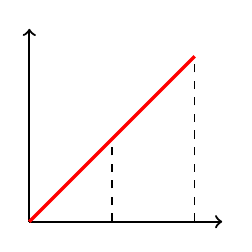
\begin{tikzpicture}[scale=0.7]
\draw[thick,->] (0,0)--(3.5,0);
\draw[thick,->] (0,0)--(0,3.5);
\draw[very thick, red] (0,0)--(3,3);
\draw[dashed] (3,0)--(3,3);
\draw[dashed] (1.5,0)--(1.5,1.5);
\end{tikzpicture}
\end{figure}

\section{Листинги}

В работах студентов кафедры <<Компьютерные технологии>> часто встречаются различные листинги. Листинги бывают
двух основных видов~--- исходный код и псевдокод. Первый оформляется с помощью окружения \texttt{lstlisting}
из пакета \texttt{listings}, который уже включается в стилевике и немного настроен. Пример Hello World на Java
приведен на листинге~\ref{lst1}.

\begin{lstlisting}[float=!h,caption={Пример исходного кода на Java},label={lst1}]
public class HelloWorld {
	public static void main(String[] args) {
		System.out.println("Hello, world!");
	}
}
\end{lstlisting}

Псевдокод можно оформлять с помощью разных пакетов. В данном стилевике включается пакет \texttt{algorithmicx}.
Сам по себе он не генерирует флоатов, поэтому для них используется пакет \texttt{algorithm}.
Пример их совместного использования приведен на листинге~\ref{lst2}. Обратите внимание, что флоаты разные, а 
нумерация~--- общая!

\begin{algorithm}[!h]
\caption{Пример псевдокода}\label{lst2}
\begin{algorithmic}
	\Function{IsPrime}{$N$}
		\For{$t \gets [2; \lfloor\sqrt{N}\rfloor]$}
			\If{$N \bmod t = 0$}
				\State\Return \textsc{false}
			\EndIf
		\EndFor
		\State\Return \textsc{true}
	\EndFunction
\end{algorithmic}
\end{algorithm}

Наконец, листинги из \texttt{listings} тоже можно подвешивать с помощью \texttt{algorithm},
пример на листинге~\ref{lst3}.

\begin{algorithm}[!h]
\caption{Исходный код и флоат \texttt{algorithm}}\label{lst3}
\begin{lstlisting}
public class HelloWorld {
	public static void main(String[] args) {
		System.out.println("Hello, world!");
	}
}
\end{lstlisting}
\end{algorithm}

\chapter{Проверка сквозной нумерации}

Листинг~\ref{lst4} должен иметь номер 4.

\begin{algorithm}[!h]
\caption{Исходный код и флоат \texttt{algorithm}}\label{lst4}
\begin{lstlisting}
public class HelloWorld {
	public static void main(String[] args) {
		System.out.println("Hello, world!");
	}
}
\end{lstlisting}
\end{algorithm}

Рисунок~\ref{fig2} должен иметь номер 2.

\begin{figure}[!h]
\caption{Пример рисунка}\label{fig2}
\centering
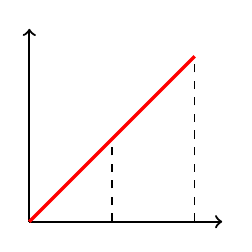
\begin{tikzpicture}[scale=0.7]
\draw[thick,->] (0,0)--(3.5,0);
\draw[thick,->] (0,0)--(0,3.5);
\draw[very thick, red] (0,0)--(3,3);
\draw[dashed] (3,0)--(3,3);
\draw[dashed] (1.5,0)--(1.5,1.5);
\end{tikzpicture}
\end{figure}

Таблица~\ref{tab3} должна иметь номер 3.

\begin{table}[!h]
\caption{Таблица умножения с помощью \texttt{tabu} (фрагмент)}\label{tab3}
\centering
\begin{tabu}{|*{18}{X[c]|}}\hline
-- & 1 & 2 & 3 & 4 & 5 & 6 & 7 & 8 & 9 & 10 & 11 & 12 & 13 & 14 & 15 & 16 & 17 \\\hline
1  & 1 & 2 & 3 & 4 & 5 & 6 & 7 & 8 & 9 & 10 & 11 & 12 & 13 & 14 & 15 & 16 & 17 \\\hline
2  & 2 & 4 & 6 & 8 & 10 & 12 & 14 & 16 & 18 & 20 & 22 & 24 & 26 & 28 & 30 & 32 & 34 \\\hline
3  & 3 & 6 & 9 & 12 & 15 & 18 & 21 & 24 & 27 & 30 & 33 & 36 & 39 & 42 & 45 & 48 & 51 \\\hline
4  & 4 & 8 & 12 & 16 & 20 & 24 & 28 & 32 & 36 & 40 & 44 & 48 & 52 & 56 & 60 & 64 & 68 \\\hline
\end{tabu}
\end{table}

\chapterconclusion

В конце каждой главы желательно делать выводы. Вывод по данной главе~--- нумерация работает корректно, ура!

%% Макрос для заключения. Совместим со старым стилевиком.
\startconclusionpage

В данном разделе размещается заключение.

%% Обратите внимание на heading. Без него тоже работает, но название будет другим.
\printbibliography[heading=trueHeading]

%% После этой команды chapter будет генерировать приложения, нумерованные русскими буквами.
%% \startappendices из старого стилевика будет делать то же самое
\appendix

\chapter{Пример приложения}

Пример ссылок на литературные источники: \cite{example-english, example-russian}.
\end{document}
